\documentclass{article} % For LaTeX2e
\usepackage{nips14submit_e,times}
%\usepackage{hyperref}
\usepackage{url}
%\documentstyle[nips14submit_09,times,art10]{article} % For LaTeX 2.09
\usepackage{natbib}
\usepackage{amsmath}
\usepackage{amsthm}
\usepackage{amssymb}
\usepackage{graphicx}
\usepackage{xspace}
\usepackage{tabularx}
\usepackage{ownstyles}

%\usepackage{xr} % to refer to external references from the main paper
%\externaldocument{main}

%\usepackage[usenames]{color} 
\newcommand{\todo}[1]{\textcolor{red}{[#1]}} %to make the ToDo Command


%\newcommand{\baseB}{baseB\xspace}
\newcommand{\net}[1]{\ensuremath{\mathsf{#1}\xspace}}
\newcommand{\baseA}{\net{baseA}}
\newcommand{\baseB}{\net{baseB}}
%\newcommand{\dA}{$A$\xspace}
%\newcommand{\dB}{$B$\xspace}
\newcommand{\dA}{\net{A}\xspace}
\newcommand{\dB}{\net{B}\xspace}





%\title{Supplementary material for: Quantifying the transferability of features in deep neural networks}
\title{Supplementary material for: How transferable are features in deep neural networks?}

\renewcommand{\refname}{Supplementary References}

\author{
Taishi Nakamura$^{*1}$, 
Mayank Mishra$^{*2}$, 
Simone Tedeschi$^{*3,4}$, 
Yekun Chai$^5$ \\
\textbf{Jason T Stillerman}, 
\textbf{Felix Friedrich}$^{6,7}$, 
\textbf{Prateek Yadav}$^8$, 
\textbf{Tanmay Laud}, \\
\textbf{Vu Minh Chien}$^9$, 
\textbf{Terry Yue Zhuo}$^{10,11}$, 
\textbf{Diganta Misra}$^{12,13}$, 
\textbf{Ben Bogin}$^{14}$, \\
\textbf{Xuan-Son Vu}$^{15,16,17}$, 
\textbf{Marzena Karpinska}$^{18}$, 
\textbf{Arnav Varma Dantuluri}, 
\textbf{Wojciech Kusa}$^{33}$, \\
\textbf{Tommaso Furlanello}, 
\textbf{Rio Yokota}$^1$, 
\textbf{Niklas Muennighoff}, 
\textbf{Suhas Pai}$^{19}$, \\
\textbf{Tosin Adewumi}$^{20}$, 
\textbf{Veronika Laippala}, 
\textbf{Xiaozhe Yao}$^{21}$, 
\textbf{Adalberto Junior}, \\
\textbf{Alpay Ariyak}$^{22,23}$, 
\textbf{Aleksandr Drozd}$^{24}$, 
\textbf{Jordan Clive}$^{25}$, 
\textbf{Kshitij Gupta}$^{12}$, \\
\textbf{Liangyu Chen}, 
\textbf{Qi Sun}$^1$, 
\textbf{Ken Tsui}, 
\textbf{Noah Persaud}, \\
\textbf{Nour Fahmy}, 
\textbf{Tianlong Chen}$^8$, 
\textbf{Mohit Bansal}$^8$, 
\textbf{Nicolò Monti}$^{26}$, \\
\textbf{Tai Dang}$^{18}$, 
\textbf{Ziyang Luo}$^{27}$, 
\textbf{Tien-Tung Bui}$^{28}$, 
\textbf{Roberto Navigli}$^3$, \\
\textbf{Virendra Mehta}$^{29}$, 
\textbf{Matthew Blumberg}$^{\#30}$, 
\textbf{Victor May}$^{\#31,32}$, 
\textbf{Huu Nguyen}$^{\#32}$, \\
\textbf{Sampo Pyysalo}$^{\#34}$ \\[1ex]
$^1$Institute of Science Tokyo,
$^2$MIT-IBM Watson Lab,
$^3$Sapienza University of Rome,\\
$^4$Babelscape,
$^5$LAION,
$^6$TU Darmstadt,
$^7$hessian.AI,
$^8$UNC Chapel-Hill \\
$^9$Detomo Inc.,
$^{10}$CSIRO's Data61,
$^{11}$Monash University,
$^{12}$Mila - Quebec AI Institute \\
$^{13}$Carnegie Mellon University,
$^{14}$Allen Institute for AI,
$^{15}$DeepTensor AB,\\
$^{16}$WASP Media \& Language,
$^{17}$Umeå University,
$^{18}$University of Massachusetts Amherst,\\
$^{19}$Hudson Labs,
$^{20}$Luleå University of Technology,
$^{21}$ETH Zurich,
$^{22}$RunPod,
$^{23}$OpenChat, \\
$^{24}$RIKEN CCS,
$^{25}$Chattermill AI,
$^{26}$ASC27,
$^{27}$Hong Kong Baptist University,
$^{28}$DopikAI JSC \\
$^{29}$University of Trento,
$^{30}$GridRepublic,
$^{31}$Chegg,
$^{32}$Ontocord.AI,
$^{33}$TU Wien,
$^{34}$University of Turku \\[1ex]
\texttt{taishi@rio.scrc.iir.isct.ac.jp},
\texttt{mayank.mishra2@ibm.com}, \\
\texttt{tedeschi@diag.uniroma1.it},
\texttt{praty@cs.unc.edu} \\
\texttt{diganta.misra@mila.quebec},
\texttt{mayvic@gmail.com}, \\
\texttt{s.vu@deeptensor.ai},
\texttt{huu@ontocord.ai},
\texttt{sampo.pyysalo@utu.fi} \\[1ex]
\texttt{\small $^*$Equal contribution \quad $^\#$Equal mentoring}
}
\vspace{10cm}



% The \author macro works with any number of authors. There are two commands
% used to separate the names and addresses of multiple authors: \And and \AND.
%
% Using \And between authors leaves it to \LaTeX{} to determine where to break
% the lines. Using \AND forces a linebreak at that point. So, if \LaTeX{}
% puts 3 of 4 authors names on the first line, and the last on the second
% line, try using \AND instead of \And before the third author name.

\newcommand{\fix}{\marginpar{FIX}}
\newcommand{\new}{\marginpar{NEW}}

\nipsfinalcopy % Uncomment for camera-ready version




% Supplementary Information hacks from http://jshodges.com/index.php?qs=kb_001
% For section headers starting with S
\renewcommand{\thesection}{S.\arabic{section}}
\renewcommand{\thesubsection}{\thesection.\arabic{subsection}}
 


\newcommand{\beginsupplementary}{%
        \setcounter{table}{0}
        \renewcommand{\thetable}{S\arabic{table}}%
        \setcounter{figure}{0}
        \renewcommand{\thefigure}{S\arabic{figure}}%
     }



\begin{document}

\beginsupplementary

\maketitle

%\begin{abstract}
%Scaling Transformers to longer sequence lengths has been a major problem in the
last several years, promising to improve performance in language modeling and
high-resolution image understanding, as well as to unlock new applications in
code, audio, and video generation.
The attention layer is the main bottleneck in scaling to longer sequences, as
its runtime and memory increase quadratically in the sequence length.
\sysnameone~\citep{dao2022flashattention} exploits the asymmetric GPU memory
hierarchy to bring significant memory saving (linear instead of quadratic) and
runtime speedup (2-4$\times$ compared to optimized baselines), with no approximation.
However, \sysnameone is still not nearly as fast as optimized matrix-multiply
(GEMM) operations, reaching only 25-40\% of the theoretical maximum FLOPs/s.
We observe that the inefficiency is due to suboptimal work partitioning between
different thread blocks and warps on the GPU, causing either low-occupancy or
unnecessary shared memory reads/writes.
We propose \sysname, with better work partitioning to address these issues.
In particular, we (1) tweak the algorithm to reduce the number of non-matmul
FLOPs (2) parallelize the attention computation, even for a single head, across
different thread blocks to increase occupancy, and (3) within each thread block,
distribute the work between warps to reduce communication through shared memory.
These yield around 2$\times$ speedup compared to \sysnameone, reaching 50-73\% of the
theoretical maximum FLOPs/s on A100 and getting close to the efficiency of GEMM
operations.
We empirically validate that when used end-to-end to train GPT-style models,
\sysname reaches training speed of up to 225 TFLOPs/s per A100 GPU (72\% model
FLOPs utilization).\footnote{\sysname
  is available at \url{https://github.com/Dao-AILab/flash-attention}}

% models with up to 2$\times$ longer sequence length compared to \sysnameone, in the
% same amount of time, leading to better downstream performance.\footnote{\sysname
%   is available at \url{https://github.com/Dao-AILab/flash-attention}}

%\end{abstract}



% !TEX root = supplementary_main.tex

\appendix



\section{Training Details}

% TODO consider fitting if possible
Since \cite{Krizhevsky-2012} won the ImageNet 2012 competition, there has naturally been much interest and work toward tweaking hyperparameters of large convolutional models. For example, \cite{Zeiler+et+al-arxiv2013b} found that it is better to decrease the first layer filters sizes from $11\times 11$ to $7\times 7$ and to use a smaller stride of $2$ instead of $4$.
However, because this study aims not for maximum absolute performance but to use 
a commonly studied architecture, we used the reference implementation provided by Caffe \citep{jia2014caffe:-convolutional-architecture}.
We followed \citet{donahue+jia-2013-arxiv} in making a few minor departures from \cite{Krizhevsky-2012} when training the convnets in this study. We skipped the data augmentation trick of adding random multiples of principle components of pixel RGB values, which produced only a $1\%$ improvement in the original paper, and instead of scaling to keep the aspect ratio and then cropping, we warped images to $256\times 256$. We also placed the Local Response Normalization layers just \emph{after} the pooling layers, instead of before them. As in previous studies, including \cite{Krizhevsky-2012}, we use dropout \citep{Hinton-et-al-arxiv2012} on fully connected layers except for the softmax output layer.

% TODO: fit this in
%For clarity of presentation, we list all hyperparameter selections in two tables: layer sizes and locations in
%\tabref{network_architecture} and weight initialization and learning rate details in
%\tabref{learning_hyperparams}. In the first table, a feedforward pass proceeds from top to bottom, left to right.

%\begin{table}[h]
%\caption{Convolutional Network architecture sizes and hyperparameters. Conv stands for Convolutional layers. FC stands for fully-connected layers. R/S indicates that the layer consists of rectilinear or sigmoidal neurons. Neurons in dropout layers fail to fire with 50\% probability \todo{accurate?} \citep{Hinton-et-al-arxiv2012}\todo{Do we need to explain what groups means? Stride?} LRN stands for local response normalization \citep{Krizhevsky-2012}.}
%\tablabel{network_architecture}
%\begin{center}
%% TODO
%% Add padding back in
%\begin{tabular}{|r|l|l|l|l|l|l|l|l|}
%\hline
%%       &      & filter & number  &        &        &     &         & Maxpool        & LRN        \\
%%name   & pad  & size   & outputs & groups & stride & R/S & Dropout & (width,stride) & (size,$\alpha$,$\beta$) \\
%%\hline
%%conv1  &      & 11x11  & 96      & 1      & 4      & R   &         & 3, 2           & 5,0.0001,0.75     \\
%%conv2  & 2    & 5x5    & 256     & 2      & 1      & R   &         & 3, 2           & 5,0.0001,0.75     \\
%%conv3  & 1    & 3x3    & 384     & 1      & 1      & R   &         &                &                   \\
%%conv4  & 1    & 3x3    & 384     & 2      & 1      & R   &         &                &                   \\
%%conv5  & 1    & 3x3    & 256     & 2      & 1      & R   &         & 3, 2           &                   \\
%%fc6    &      &        & 4096    & 1      &        & R   & *       &                &                   \\
%%fc7    &      &        & 4096    & 1      &        & R   & *       &                &                   \\
%%fc8    &      &        & 1000    & 1      &        & S   &         &                &                   \\
%        & filter & number  &        &        &     &         & Maxpool        & LRN        \\
%name    & size   & outputs & groups & stride & R/S & Dropout & (width,stride) & (size,$\alpha$,$\beta$) \\
%\hline
%conv1   & 11x11  & 96      & 1      & 4      & R   &         & 3, 2           & 5,0.0001,0.75     \\
%conv2   & 5x5    & 256     & 2      & 1      & R   &         & 3, 2           & 5,0.0001,0.75     \\
%conv3   & 3x3    & 384     & 1      & 1      & R   &         &                &                   \\
%conv4   & 3x3    & 384     & 2      & 1      & R   &         &                &                   \\
%conv5   & 3x3    & 256     & 2      & 1      & R   &         & 3, 2           &                   \\
%fc6     &        & 4096    & 1      &        & R   & *       &                &                   \\
%fc7     &        & 4096    & 1      &        & R   & *       &                &                   \\
%fc8     &        & 1000    & 1      &        & S   &         &                &                   \\
%\hline
%\end{tabular}
%\end{center}
%\end{table}

%\begin{table}[t]
%\caption{Parameter initializations and learning rates. \todo{JY: I expanded the table headings (we have the space). Please check that I did so accurately. I had to guess on most.}}
%\tablabel{learning_hyperparams}
%\begin{center}
%\begin{tabular}{|r|l|l|l|l|l|l|}
%\hline
%       & \multicolumn{3}{c|}{\bf Weight}     &  \multicolumn{3}{c|}{\bf Bias}       \\
%\cline{2-7}
%       & Gaussian Std. Dev.   & Local Response-multiplier & decay &  const  & Local Response  & decay \\
%\hline
%conv1  & .01    & 1       & y     &  0      & 2   & n     \\
%conv2  & .01    & 1       & y     &  1      & 2   & n     \\
%conv3  & .01    & 1       & y     &  0      & 2   & n     \\
%conv4  & .01    & 1       & y     &  1      & 2   & n     \\
%conv5  & .01    & 1       & y     &  1      & 2   & n     \\
%fc6    & .005   & 1       & y     &  1      & 2   & n     \\
%fc7    & .005   & 1       & y     &  1      & 2   & n     \\
%fc8    & .01    & 1       & y     &  0      & 2   & n     \\ 
%\hline
%\end{tabular}
%\end{center}
%\end{table}

% TODO: reinsert
We trained with stochastic gradient descent (SGD) with momentum. Each iteration of SGD used a batch size of 256, a momentum of 0.9, and a multiplicative weight decay (for those weights with weight decay enabled, i.e. not for frozen weights) of 0.0005 per iteration.
The master learning rate started at 0.01, and annealed over the course of training by dropping by a factor of 10 every 100,000 iterations. Learning stopped after 450,000 iterations.
Each iteration took about {\raise.17ex\hbox{$\scriptstyle\sim$}}1.7 seconds on a NVidia K20 GPU, meaning the whole training procedure for a single network took {\raise.17ex\hbox{$\scriptstyle\sim$}}9.5 days.

%Because occupying a whole GPU for this long was cumbersome, we also devised a set of hyperparameters to allow faster learning by boosting the learning rate by 25\% to 0.0125, annealing by a factor of 10 after only 64,000 iterations, and stopping after 200,000 iterations. These selections were made after looking at the learning curves for the base case and estimating at which points in each region of constant learning rate the learning had plateaued and thus annealing could take place.
%This faster training schedule was only used for the natural vs. man-made experiments in \secref{experiments_random_nm}.

%\edit{A typical learning curve is shown in \figref{typical_learning}.}
%
%\editbox{
%Figure {typical\_learning}
%(( make this figure, if important, once reduced-1300-2 run is done ))
%}

Our base model attains a final top-1 error on the validation set of 42.5\%, about the same as the 42.9\% reported by \cite{donahue+jia-2013-arxiv} and 1.8\% worse than \cite{Krizhevsky-2012}, the latter difference probably due to the few minor training differences explained above. We checked these values only to demonstrate that the network was converging reasonably. As our goal is not to improve the state of the art, but to investigate the properties of transfer, small differences in raw performance are not of concern.

Because code is often more clear than text, we've also made all code and parameter files necessary to reproduce these experiments available on
\url{http://yosinski.com/transfer}.



\section{How Much Does an AlexNet Architecture Overfit?}
\seclabel{supp_overfit}

\begin{figure}[th]
\begin{center}
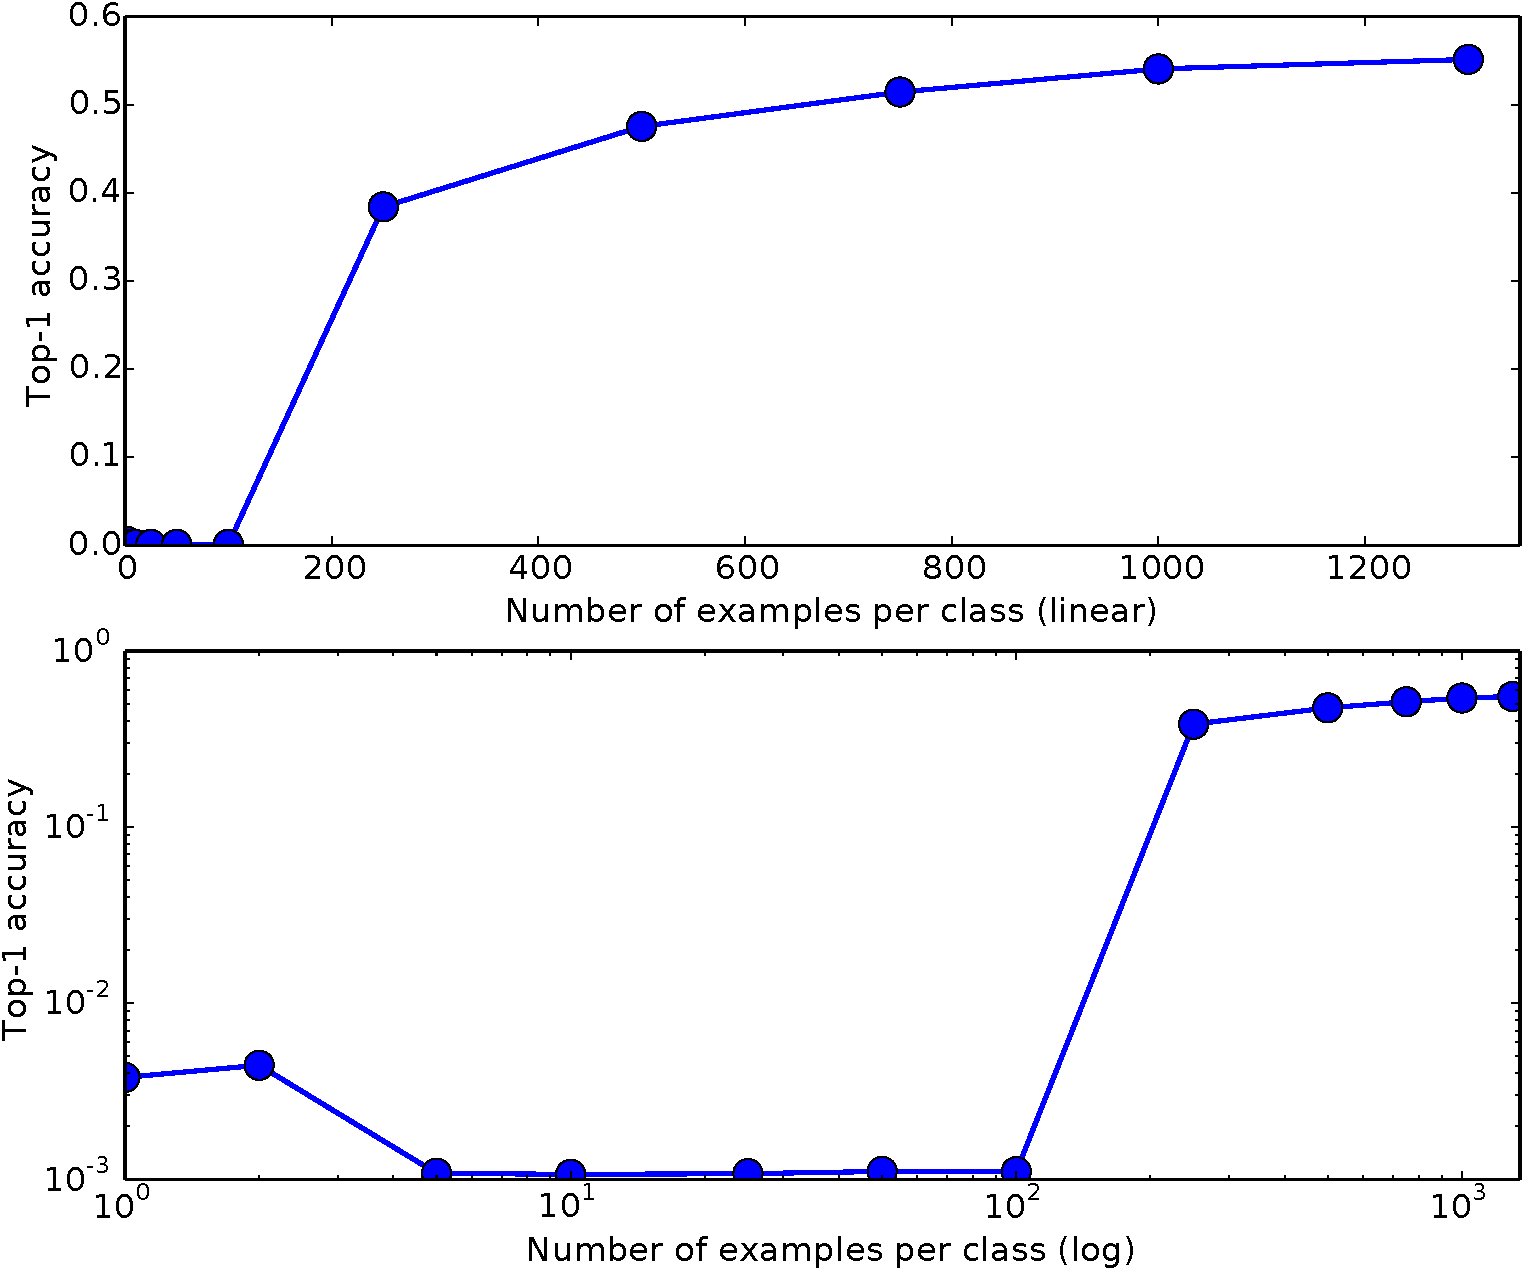
\includegraphics[width=1.0\linewidth]{plots/result_reduced_crop.pdf}
\end{center}
\caption{Top-1 validation accuracy for networks trained on datasets containing reduced numbers of examples. The largest dataset contains the entire ILSVRC2012 \citep{imagenet_cvpr09} release with a maximum of 1300 examples per class, and the smallest dataset contains only 1 example per class (1000 data points in total). \emph{Top}: linear axes. The slope of the rightmost line segment between 1000 and 1300 is nearly zero, indicating that the amount of overfit is slight. In this region the validation accuracy rises by 0.010820 from 0.54094 to 0.55176. \emph{Bottom}: logarithmic axes. It is interesting to note that even the networks trained on a single example per class or two examples per class manage to attain 3.8\% or 4.4\% accuracy, respectively. Networks trained on \{5,10,25,50,100\} examples per class exhibit poor convergence and attain only chance level performance.}
\figlabel{reduced}
\end{figure}

We observed relatively poor
performance of random filters in an AlexNet
architecture \citep{Krizhevsky-2012} trained on ImageNet, which is in contrast to previously reported successes with random
filters in a smaller convolutional networks
trained on the smaller Caltech-101 dataset \citep{Jarrett-ICCV2009}.
One hypothesis presented in the main paper is that this difference is observed because ImageNet is large
enough to support training an AlexNet architecture without excessive overfitting.
We sought to support or disprove this hypothesis by creating reduced
size datasets containing the same 1000 classes as ImageNet, but where
each class contained a maximum of $n$ examples, for each $n \in \{1300 ,1000 ,750
,500 ,250 ,100 ,50 ,25 ,10 ,5 ,2 ,1\}$. The case of $n = 1300$ is the
complete ImageNet dataset.

Because occupying a whole GPU for this long was infeasible given our available computing resources, we also
devised a set of hyperparameters to allow faster learning by boosting
the learning rate by 25\% to 0.0125, annealing by a factor of 10 after
only 64,000 iterations, and stopping after 200,000 iterations. These
selections were made after looking at the learning curves for the base
case and estimating at which points learning had plateaued and thus annealing could take
place.  This faster training schedule was only used for the
experiments in this section. Each run took just over 4 days on a K20
GPU.

\begin{table}[th]
\caption{An enumeration of the points in \figref{reduced} for clarity.}
\tablabel{reduced}
\begin{center}
\begin{tabular}{|r|l|}
\hline
Number        & Top-1 \\
 of examples  & validation \\
per class           & accuracy \\
\hline
1300  &  0.55176  \\
1000  &  0.54094  \\
750   &  0.51470   \\
500   &  0.47568   \\
250   &  0.38428   \\
100   &  0.00110   \\
50    &  0.00111   \\
25    &  0.00107   \\
10    &  0.00106   \\
5     &  0.00108   \\
2     &  0.00444   \\
1     &  0.00379   \\
\hline
\end{tabular}
\end{center}
\end{table}

The results of this experiment are shown in \figref{reduced}
and \tabref{reduced}. The rightmost few points in the top subplot
of \figref{reduced} appear to converge, or nearly converge, to an
asymptote, suggesting that validation accuracy would not improve
significantly when using an AlexNet model with much more data, and
thus, that the degree of overfit is not severe.



\section{Man-made vs. Natural Split}
\seclabel{supp_natman}

In order to compare transfer performance between tasks \dA and \dB
such that \dA and \dB are as semantically dissimilar as possible, we
sought to find two disjoint subsets of the 1000 classes in ImageNet
that were as unrelated as possible. To this end we annotated each node
$x_i$ in the WordNet graph with a label $n_i$ such that $n_i$ is the
number of distinct ImageNet classes reachable by starting at $x_i$ and traversing the graph only in the parent
$\rightarrow$ child direction.
The 20 nodes with largest $n_i$ are the following:

{
\small
\begin{verbatim}
 n_i   x_i
1000   n00001740: entity
 997   n00001930: physical entity
 958   n00002684: object, physical object
 949   n00003553: whole, unit
 522   n00021939: artifact, artefact
 410   n00004475: organism, being
 410   n00004258: living thing, animate thing
 398   n00015388: animal, animate being, beast, brute, creature, fauna
 358   n03575240: instrumentality, instrumentation
 337   n01471682: vertebrate, craniate
 337   n01466257: chordate
 218   n01861778: mammal, mammalian
 212   n01886756: placental, placental mammal, eutherian, eutherian mammal
 158   n02075296: carnivore
 130   n03183080: device
 130   n02083346: canine, canid
 123   n01317541: domestic animal, domesticated animal
 118   n02084071: dog, domestic dog, Canis familiaris
 100   n03094503: container
  90   n03122748: covering
\end{verbatim}
}

Starting from the top, we can see that the largest subset, \texttt{entity}, contains all
1000 ImageNet categories. Moving down several items, the first
subset we encounter containing approximately half of the classes
is \texttt{artifact} with 522 classes. The next is \texttt{organism}
with 410. Fortunately for this study, it just so happens that these two subsets are mutually
exclusive, so we used the first to populate our \textit{man-made} category and the second to populate our \textit{natural} category.
 There are
$1000 - 522 - 410 = 68$ classes remaining outside these two subsets, and we manually assigned these to either category as seemed more appropriate.
For example, we placed
\texttt{pizza}, 
\texttt{cup}, and
\texttt{bagel} into \textit{man-made} and 
\texttt{strawberry}, 
\texttt{volcano}, and 
\texttt{banana} into \textit{natural}. This process results in 551 and 449 classes, respectively. The 68 manual decisions are shown below, and the complete list of 551 man-made and 449 natural classes is available at \url{http://yosinski.com/transfer}.


\pagebreak

Classes manually placed into the man-made category:
{
\scriptsize
\begin{verbatim}
n07697537 hotdog, hot dog, red hot
n07860988 dough
n07875152 potpie
n07583066 guacamole
n07892512 red wine
n07614500 ice cream, icecream
n09229709 bubble
n07831146 carbonara
n07565083 menu
n07871810 meat loaf, meatloaf
n07693725 bagel, beigel
n07920052 espresso
n07590611 hot pot, hotpot
n07873807 pizza, pizza pie
n07579787 plate
n06874185 traffic light, traffic signal, stoplight
n07836838 chocolate sauce, chocolate syrup
n15075141 toilet tissue, toilet paper, bathroom tissue
n07613480 trifle
n07880968 burrito
n06794110 street sign
n07711569 mashed potato
n07932039 eggnog
n07695742 pretzel
n07684084 French loaf
n07697313 cheeseburger
n07615774 ice lolly, lolly, lollipop, popsicle
n07584110 consomme
n07930864 cup
\end{verbatim}
}

Classes manually placed into the natural category:

{
\scriptsize
\begin{verbatim}
n13133613 ear, spike, capitulum
n07745940 strawberry
n07714571 head cabbage
n09428293 seashore, coast, seacoast, sea-coast
n07753113 fig
n07753275 pineapple, ananas
n07730033 cardoon
n07749582 lemon
n07742313 Granny Smith
n12768682 buckeye, horse chestnut, conker
n07734744 mushroom
n09246464 cliff, drop, drop-off
n11879895 rapeseed
n07718472 cucumber, cuke
n09468604 valley, vale
n07802026 hay
n09288635 geyser
n07720875 bell pepper
n07760859 custard apple
n07716358 zucchini, courgette
n09332890 lakeside, lakeshore
n09193705 alp
n09399592 promontory, headland, head, foreland
n07717410 acorn squash
n07717556 butternut squash
n07714990 broccoli
n09256479 coral reef
n09472597 volcano
n07747607 orange
n07716906 spaghetti squash
n12620546 hip, rose hip, rosehip
n07768694 pomegranate
n12267677 acorn
n12144580 corn
n07718747 artichoke, globe artichoke
n07753592 banana
n09421951 sandbar, sand bar
n07715103 cauliflower
n07754684 jackfruit, jak, jack
\end{verbatim}
}


%% !TEX root = main.tex

\section*{Acknowledgments}

\vspace*{-1ex}

The authors would like to thank Kyunghyun Cho and Thomas Fuchs for helpful discussions, Joost Huizinga, Anh Nguyen, and Roby Velez for editing, as well as funding from 
the NASA Space Technology Research Fellowship (JY), DARPA project W911NF-12-1-0449, NSERC, Ubisoft, and CIFAR
(YB is a CIFAR Fellow).



\pagebreak

%{\small
%\bibliography{strings,strings-shorter,ml,aigaion-shorter,cultrefs}
\bibliography{lisa_ml,bibdesk}
\bibliographystyle{natbib}
%}

\end{document}
